\documentclass[12pt]{article}
\usepackage{amsmath}
\usepackage{mathtools}
\usepackage{bigints}
\usepackage{parskip}
\usepackage{amssymb}
\usepackage{relsize}
\usepackage{fullpage}
% \DeclareMathSizes{12}{17.28}{9}{7} % (a)

\DeclareMathSizes{12}{17.28}{12}{12} % (a)


\usepackage{hyperref}



	\addtolength{\topmargin}{-.5in}
	\addtolength{\textheight}{1.75in}



    \newenvironment{myindentpar}[1]%
     {\begin{list}{}%
             {\setlength{\leftmargin}{#1}}%
             \item[]%
     }
     {\end{list}}

\begin{document}
\title{College Algebra: Module 5 What You Need To Know}
\date{2-12-15}
\author{}
\maketitle


\section{Complex Numbers (Section 1.4)}

\textbf{Complex Numbers} - \textit{Complex Numbers} are numbers that can be written in the form 
\newline

\centerline{$a + bi$} 

\hspace{4cm} where $a$ and $b$ are real numbers and $i$ is the imaginary unit
\newline

\textbf{Imaginary Unit:} $i = \sqrt{-1}$ and $i^{2} = -1$
\newline

\textbf{Property 1:} $\sqrt{-k} = i \sqrt{k}$ \hspace{1cm} ($k > 0$)
\newline

\textbf{Algebraic Rules:}

\begin{enumerate}

\item \textbf{Addition/Subtraction:} $(a + bi) \pm (c+di) = (a \pm c) + (b \pm d)i$
\item \textbf{Multiplication:} $(a + bi) \cdot (c+di) = (ac - bd) + (bc + ad)i$
\item \textbf{Division:} $\dfrac{a+bi}{c+di} = \dfrac{a + bi}{c+di} \cdot \dfrac{c-di}{c-di}$
\newline

 \hspace{3.6cm} $= \dfrac{(ac + bd) + (bc - ad)i}{c^2 + d^2}$ 

\end{enumerate}

\textbf{Note:} To divide two complex numbers you need to multiply the top and bottom by the \textbf{conjugate} of the bottom. 



\section{Solving Quadratic Equations (Section 1.5)}

\textbf{Quadratic Equation} - a \textit{quadratic equation} is an equation of the form
\newline

\centerline{$ax^{2} + bx  + c$}

\hspace{4.2cm} where $a,b,c$ are all real numbers and $a \neq 0$

\textbf{Zero Product Property:} $A \cdot B = 0 \implies A = 0$ or $B = 0$

\textbf{Square Root Property of Equality:} $x^{2} = a \implies x = \pm \sqrt{a}$ 
\newline

\textbf{Completing The Square:} In order to solve equations of the following form
\newline

\centerline{$ax^{2} + bx + c = 0$}

\hspace{5cm} by \textit{completing the square} we follow these steps:
\newline

\begin{enumerate}
\item Subtract the constant $c$ from both sides
\item Divide both sides by $a$
\item Compute $\Big(\dfrac{b}{2a}\Big)^2$ and add the result to both sides
\item Factor left hand side and simplify right hand side
\item Solve using the square root property of equality 
\end{enumerate}

\vspace{1cm}

\textbf{Quadratic Formula:} 

\centerline{$x = \dfrac{-b \pm \sqrt{b^{2} - 4ac}}{2a}$}

\vspace{1cm}

\textbf{Discriminant of the Quadratic Formula:} Given a quadratic
\newline

\centerline{$ax^{2} + bx + c$}

where $a \neq 0$ then we can determine the number and type of solutions to 
\newline

\centerline{$ax^{2} + bx + c = 0$}

by examining the discriminant of the quadratic formula which is given by 
\newline

\centerline{$b^{2} - 4ac$}

 (i.e. the terms underneath the square root in the quadratic formula) The rules are given below:

\begin{enumerate}

\item $b^2 - 4ac > 0 \implies $ 2 real roots
\item $b^2 - 4ac = 0 \implies $ 1 real (repeated) root
\item $b^2 - 4ac < 0 \implies $ 2 nonreal roots

\end{enumerate}

\newpage

\textbf{Problem 1:} Write the quadratic equation whose roots are $-2$ and $6$ and whose leading coefficient is $3$

\vspace{2cm}

\textbf{Problem 2:} Write the quadratic equation whose roots are $1$ and $6$ and whose leading coefficient is $4$

\vspace{2cm}

\textbf{Problem 3:} The length of a rectangle is $7$ ft leass than three times the width. The area of the rectangle is $66$ ft. Find the dimensions of the rectangle.

\vspace{2cm}

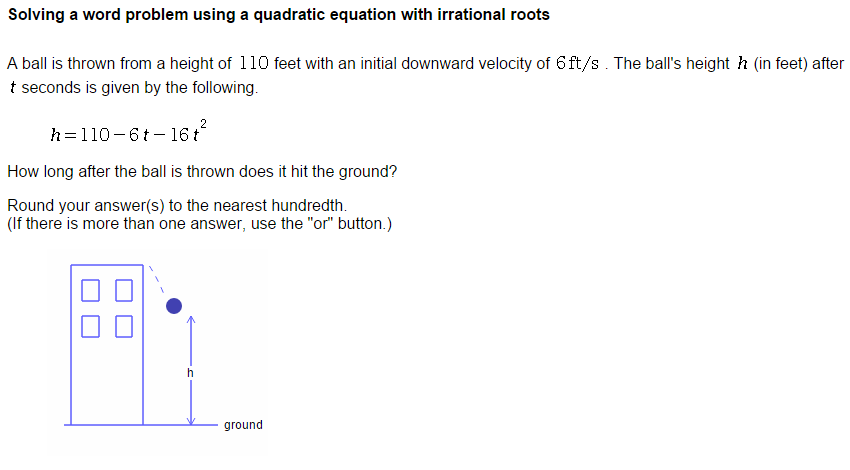
\includegraphics[scale = 0.8]{WP.png}












































\end{document}